% Lu's Task 1 working copy. The original file is R2R.tex.
% LaTeX rebuttal letter example.
% 2018 fzenke.net
\documentclass[11pt]{article}
\usepackage{comment}
\usepackage{booktabs}
\usepackage{enumitem}
% \usepackage[style=authoryear,maxcitenames=2]{biblatex}
\usepackage{lipsum} % to generate some filler text
\usepackage{fullpage}
\usepackage{amsmath}
\usepackage{amssymb}
% \usepackage{natbib}
\usepackage{tikz}
\usepackage{bbding}
\usepackage{caption}
\usepackage{tabularx}
\usepackage{makecell}

% \usepackage[normalem]{ulem}
\usepackage{color,soul}
\usepackage[colorinlistoftodos,prependcaption,textsize=footnotesize, color=lightgray]{todonotes}
\usepackage{float}
\usepackage{csquotes}
\usepackage{xcolor}
\usepackage{soul}
\usepackage[markup=underlined,commandnameprefix=ifneeded]{changes}
% \usepackage{amsthm}
\PassOptionsToPackage{hyphens}{url}
\usepackage[colorlinks=true,linkcolor=blue,citecolor=blue]{hyperref}
\hypersetup{
    colorlinks=true,
    linkcolor=blue,
    filecolor=magenta,      
    urlcolor=cyan,
}
\usepackage[most]{tcolorbox}
\tcbuselibrary{breakable}
\tcbset {
  base/.style={
    arc=0mm, 
    bottomtitle=0.5mm,
    boxrule=0mm,
    colbacktitle=black!10!white, 
    coltitle=black, 
    fonttitle=\bfseries, 
    left=2.5mm,
    leftrule=1mm,
    right=3.5mm,
    title={#1},
    toptitle=0.75mm, 
  }
}

\definecolor{brandblue}{rgb}{0.34, 0.7, 1}
\newtcolorbox{mainbox}[1]{
  colframe=lightgray,
  breakable,
  base={#1}
}

\newtcolorbox{subbox}[1]{
  colframe=black!30!white,
  base={#1}
}
\tcbuselibrary{listings}

\newtcblisting{mainboxverb}{
  colframe=lightgray,
  colback=white,
  listing only,
  breakable,
  listing options={
    basicstyle=\ttfamily\small,
    breaklines=true
  }
}
\usepackage{xcolor}
\usepackage{fancyvrb}
\DefineVerbatimEnvironment{shadedverbatim}{Verbatim}{
  breaklines=true,
  fontsize=\small,
  bgcolor=gray!12
}
\setlength{\marginparwidth}{2cm}

\usepackage{graphicx}
\usepackage{subcaption}

\usepackage{multirow}

\usepackage{mathtools}
\usepackage{adjustbox} %
% import Eq and Section references from the main manuscript where needed
% \usepackage{xr}
% \externaldocument{manuscript}

% package needed for optional arguments
\usepackage{xifthen}
\newcommand{\tw}[1]{\textcolor{red}{[TW: #1]}}

\usepackage{natbib}
 % \bibpunct[, ]{(}{)}{,}{a}{}{,}% g
 % \def\bibfont{\small}%
 % \def\bibsep{\smallskipamount}%
 % \def\bibhang{24pt}% -
 % \def\newblock{\ }%
 % \def\BIBand{and}%
\usepackage{caption}

 \newenvironment{general}
 {\par\medskip \noindent \begin{sf}\textbf{Reply}:\ }
 {\medskip \end{sf}}
 \setlength{\parskip}{10pt}

% SE Counter
\newcounter{se}[section]
\newenvironment{se}[1][]{%
    \refstepcounter{se}\par\medskip\noindent%
    \textbf{SE \these: #1}\rmfamily\itshape%
}{\medskip}

\newenvironment{se*}[1][]{%
    \par\medskip%
    \rmfamily\itshape%
}{\medskip}


% AE Counter
\newcounter{aed}[section]
\newenvironment{aed}[1][]{%
    \refstepcounter{aed}\par\medskip\noindent%
    \textbf{AE \theaed: #1}\rmfamily\itshape%
}{\medskip}
 \setlength{\parskip}{10pt}

\newenvironment{aed*}[1][]{%
    \par\medskip%
    \rmfamily\itshape%
}{\medskip}
\setlength{\parskip}{10pt}


% define counters for reviewers and their points
\newcounter{reviewer}
\setcounter{reviewer}{0}
\newcounter{point}[reviewer]
\setcounter{point}{0}


% This refines the format of how the reviewer/point reference will appear.






\renewcommand{\thepoint}{R\,\thereviewer.\arabic{point}}

% command declarations for reviewer points and our responses

\newcommand{\sesection}
{\newpage
\section*{Response to the Senior Editor}}



\newcommand{\aesection}
{\newpage
\section*{Response to the Associate Editor}}


\newcommand{\reviewersection}{\stepcounter{reviewer} \newpage
 \section*{Response to Reviewer \thereviewer}}

\newenvironment{point}{
    \refstepcounter{point} \bigskip \noindent {\textbf{\thepoint}}: \rmfamily \itshape
}{\medskip}
\setlength{\parskip}{10pt}

\newenvironment{point*}{\bigskip \noindent \rmfamily \itshape}{\medskip} % chktex 6
\setlength{\parskip}{10pt}

\newcommand{\shortpoint}[1]{\refstepcounter{point} \bigskip \noindent
{\textbf{\thepoint}} ---~#1\par }

\newenvironment{reply}
 {\par\medskip \noindent \begin{sf}\textbf{Reply}:\ }
 {\medskip \end{sf}}
 \setlength{\parskip}{10pt}

\newcommand{\shortreply}[2][]{%
    \medskip \noindent
    \begin{sf}\textbf{Reply}:\ #2
        \ifthenelse{\equal{#1}{}}{}{ \hfill \footnotesize (#1)}%
        \medskip
    \end{sf}
}

% \addbibresource{Neurips2024/LLMref.bib}

\begin{document}
\begin{sf}

\flushleft{}
\today
\vspace{15pt}

Professor Hemant Bhargava\\
Department Editor\\
\textit{Management Science}\\
\vspace{15pt}

Dear Professor Bhargava,\\
\vspace{20pt}

We sincerely thank you and the review team for the thoughtful and constructive feedback on our manuscript, and we greatly appreciate the opportunity to revise and resubmit our work under a \textbf{major revision} decision. The reviewers' comments were extremely valuable, and we took them very seriously. In the revised manuscript, we have addressed all comments and concerns raised, and we believe the paper has benefited significantly from this process.

For ease of review, we provide a detailed Summary of Major Changes at the beginning of the revised manuscript. We hope the revised paper addresses the concerns raised and clarifies the paper's contribution.

We appreciate your time and consideration and look forward to your feedback on this revision.

\vspace{10pt}

Best regards\\
The Authors

\newpage
\textbf{\Large Summary of Major Changes}\label{sec:majorchanges}

\tw{To be completed after the revision.}

\end{sf}

\newpage

% \textsf{For ease of reference, we copy your original comments here, in \emph{italics} font.}

\sesection{}

\begin{se*}

Thank you for submitting your revised paper to Management Science. Attached please find evaluation reports from three reviewers and an Associate Editor. The review team appreciates the hard work you've put into the revision, and there is a general sense of progress, although the review team still raises too many concerns for this stage of the paper. The AE report synthesizes these concerns and likely next steps: items 1 and 5 seem direct to address (improve clarity, remove inconsistencies); items 2 and 3 are crucial in the next step because they relate to conceptual/definitional issues in setting up the contribution (what exactly is the benchmark and what would be a good answer look like), and in establishing novelty relative to prior work (what this paper adds to known critiques of SHAP, LIME). And in item 4, the AE helpfully suggests a possible positive path.

\end{se*}

\begin{reply}

\end{reply}


\begin{se}
Overall, I would have liked a more definitive movement towards Accept/Reject in this round. However, given the potential to make such a contribution (but it is not evident yet) I will go along with the AE and invite you to submit another revision. It will be crucial for this version to establish a more solid contribution and impact, but the AE and I are hopeful you can get there with a careful rethinking and writing. Good luck!

\end{se}

\begin{reply}

\end{reply}


\begin{se*}

Your next revision will be crucial, and it needs to be comprehensive and successful at addressing the concerns (and of course also reflect on additional details in the reviewers' reports). I wish you the best in this effort.

\end{se*}


\vspace*{0.5\baselineskip}

\textsf{Thank you again for the opportunity to revise our paper! We are grateful to the constructive feedback from the review team. We hope that this revision satisfactorily addresses the concerns of the review team.}

\aesection{}
\begin{se*}
This revision went back to the three original reviewers. All of the reviewers find this revision significantly improved, and I agree with them. There is much to like about this revision, and the paper is shaping up to be a very impactful one. Having said that, the reviewers also had lots of comments and suggestions that need to be resolved and would make the paper even better. There are several overlapping concerns and suggested improvements that I also share. I focus on the five most important points below, but please respond and address the review team's concerns not highlighted here.
\end{se*}

\begin{reply}

\end{reply}


\begin{aed}
The paper needs to be clearer about what exactly is failing. At different points, the problem seems to arise from the predictive model, limits in what the data can identify, or the post hoc explainer. These are related issues, but they are not the same. The paper also needs to be precise about whether the relationship between $\mathbf{X}$ and $Y$ is associational or causal. This distinction affects the central claim, the interpretation of the results, and the contribution of the paper.
\end{aed}

\begin{reply}
{\color{red}
The revised manuscript separates the three candidate sources of misalignment---approximation error ($\mathcal{M}\neq\mathcal{G}$), identification failure (predictive accuracy does not pin down attribution), and explainer-induced distortion---and tags each empirical section by the source it isolates. The new forward marginal effects (FME) baseline anchors this decomposition empirically: FME perturbs the fitted model directly, with no explainer in the loop, so any alignment gap between FME and SHAP/LIME is attributable to the explainer layer rather than to the model or the data. Across the 81 datasets (best model per dataset), FME attains a mean direction alignment of 0.972 (median 0.975), exceeding {\color{blue}\textbf{[Task 1 modification]} SHAP (mean 0.821; median 0.823) and LIME (mean 0.717; median 0.683)} on the identical metric and the identical common ground-truth reference. The fitted models themselves recover the direction of feature effects almost perfectly; the additional direction errors documented for SHAP and LIME are introduced by the explanation layer. The revision also declares the estimand explicitly: all claims about $\mathbf{X} \mapsto Y$ are associational, ceteris paribus properties of the conditional expectation under $\mathcal{G}$.
}
\end{reply}


\begin{aed}
The paper needs a clearer basis for judging the size and meaning of the reported failures. The reviewers raise the absence of a meaningful benchmark, and I share this concern. Without a clear comparison point, it is difficult to know how much of the observed misalignment is specific to the post hoc explanation pipeline and how much reflects the broader difference between prediction and inference. It is also difficult to know when the reported levels of alignment should be considered practically adequate or inadequate. Relatedly, the paper should make the consequences of these errors more concrete. The reader needs a better sense of why the misinterpretation matters for the decisions that researchers, managers, or policymakers may make.
\end{aed}

\begin{reply}
{\color{red}
The revision adds a benchmark suite scored under the identical direction and strength metrics, on the same 81 data-generating processes and the same best-performing models: (i) OLS with standardized features---what a researcher who skipped the ML pipeline would report; (ii) partial dependence (PDP; Friedman 2001), the ML-native global-curve summary; and (iii) forward marginal effects (FME), which perturb the fitted model directly with no explainer in the loop.

\begin{center}
\begin{tabular}{lcc}
\toprule
 & Direction alignment & Strength alignment \\
Method & mean (median) & mean (median) \\
\midrule
OLS (standardized) & 0.758 (0.765) & 0.738 (0.779) \\
Partial dependence & 0.810 (0.815) & 0.885 (0.927) \\
Forward marginal effects & 0.972 (0.975) & 0.853 (0.903) \\
{\color{blue}\textbf{[Task 1 modification]} SHAP} & {\color{blue}0.821 (0.823)} & {\color{blue}0.864 (0.915)} \\
{\color{blue}\textbf{[Task 1 modification]} LIME} & {\color{blue}0.717 (0.683)} & {\color{blue}0.616 (0.700)} \\
\bottomrule
\end{tabular}
\end{center}
{\color{blue}\textbf{[Task 1 modification]} The SHAP/LIME entries report the exact Figure~3 means and medians under the common ground-truth target.}

{\color{blue}\textbf{[Task 1 modification]} Figure~3 has been regenerated from the finalized common-ground-truth results. The four panels used for the revised figure are provided in \texttt{Round2/figures/}:}

\begin{figure}[H]
    \centering
    \begin{subfigure}[t]{0.48\textwidth}
        \centering
        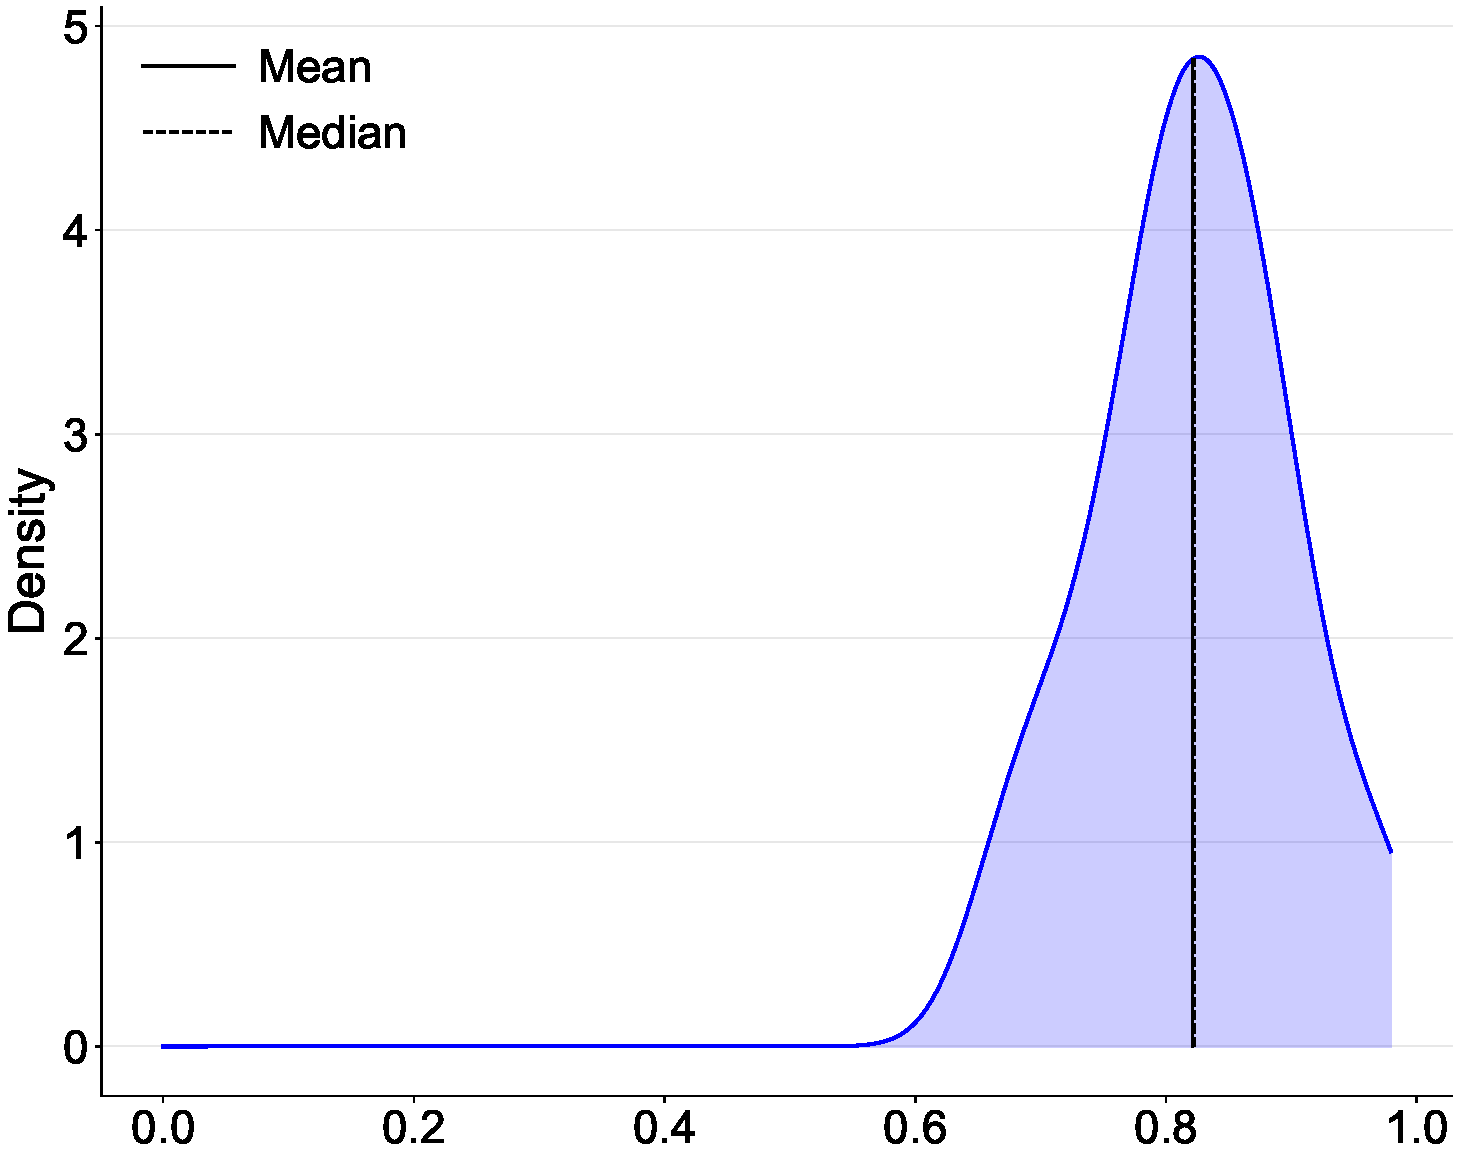
\includegraphics[width=\linewidth]{figures/shap_directionality_1.pdf}
        \caption{{\color{blue}SHAP direction alignment}}
    \end{subfigure}
    \hfill
    \begin{subfigure}[t]{0.48\textwidth}
        \centering
        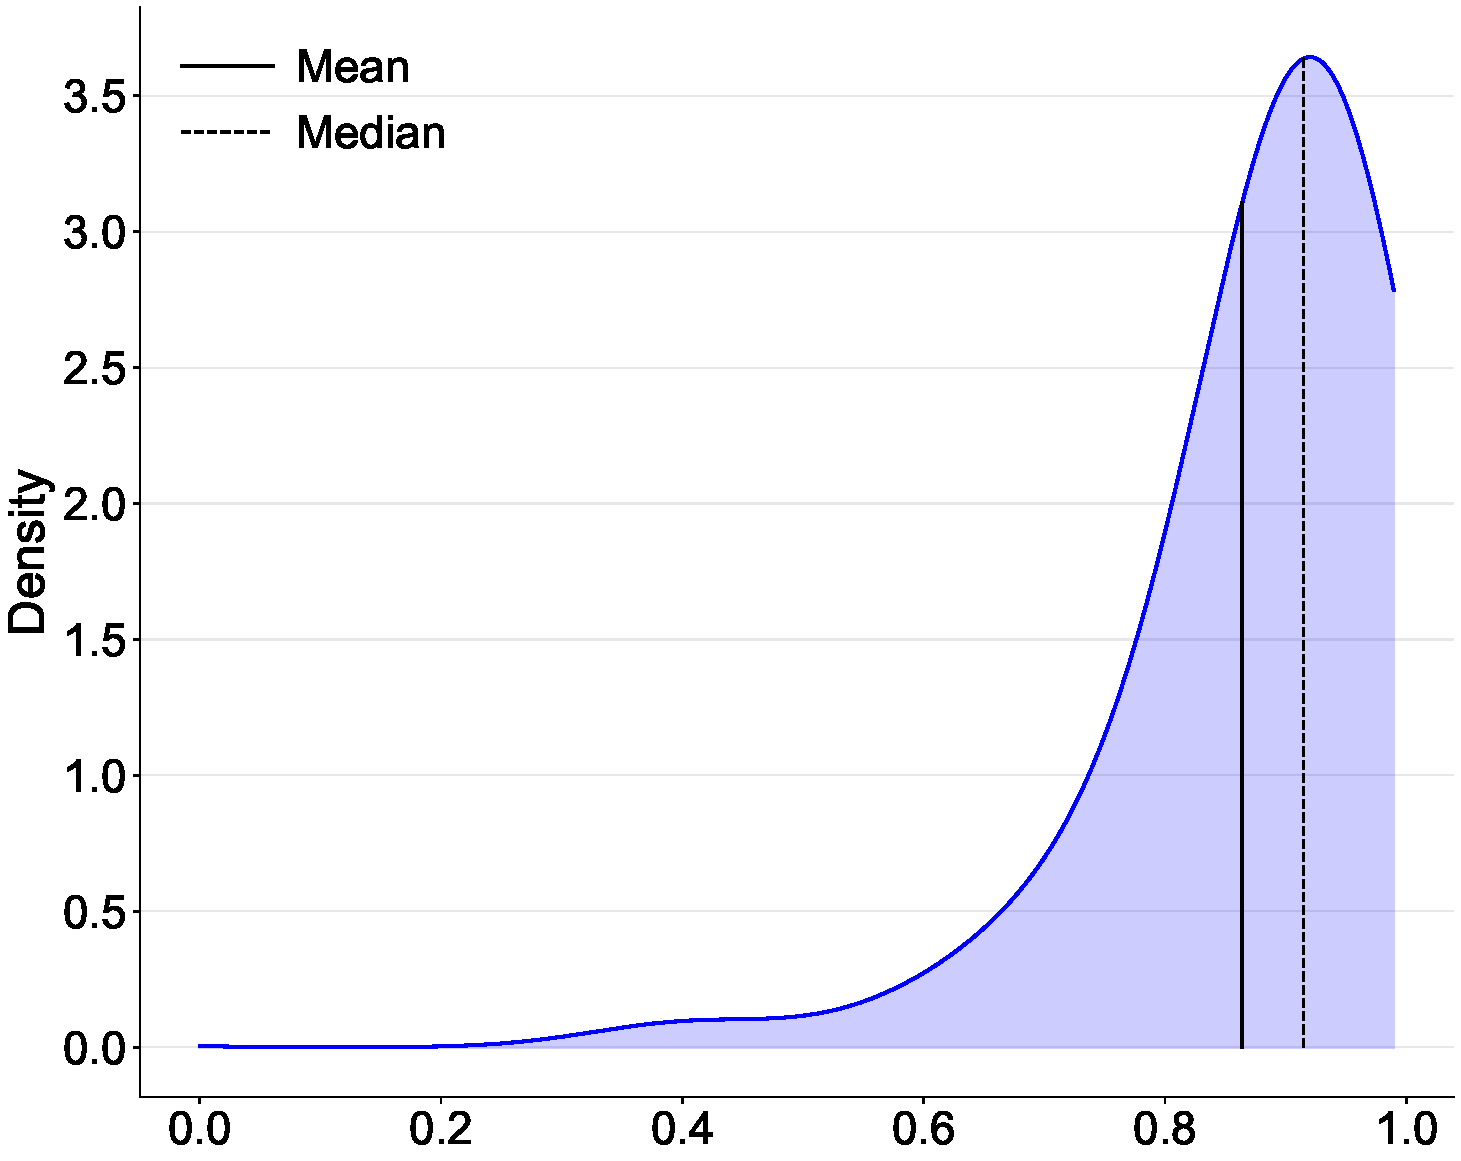
\includegraphics[width=\linewidth]{figures/shap_strength_1.pdf}
        \caption{{\color{blue}SHAP strength alignment}}
    \end{subfigure}
    \begin{subfigure}[t]{0.48\textwidth}
        \centering
        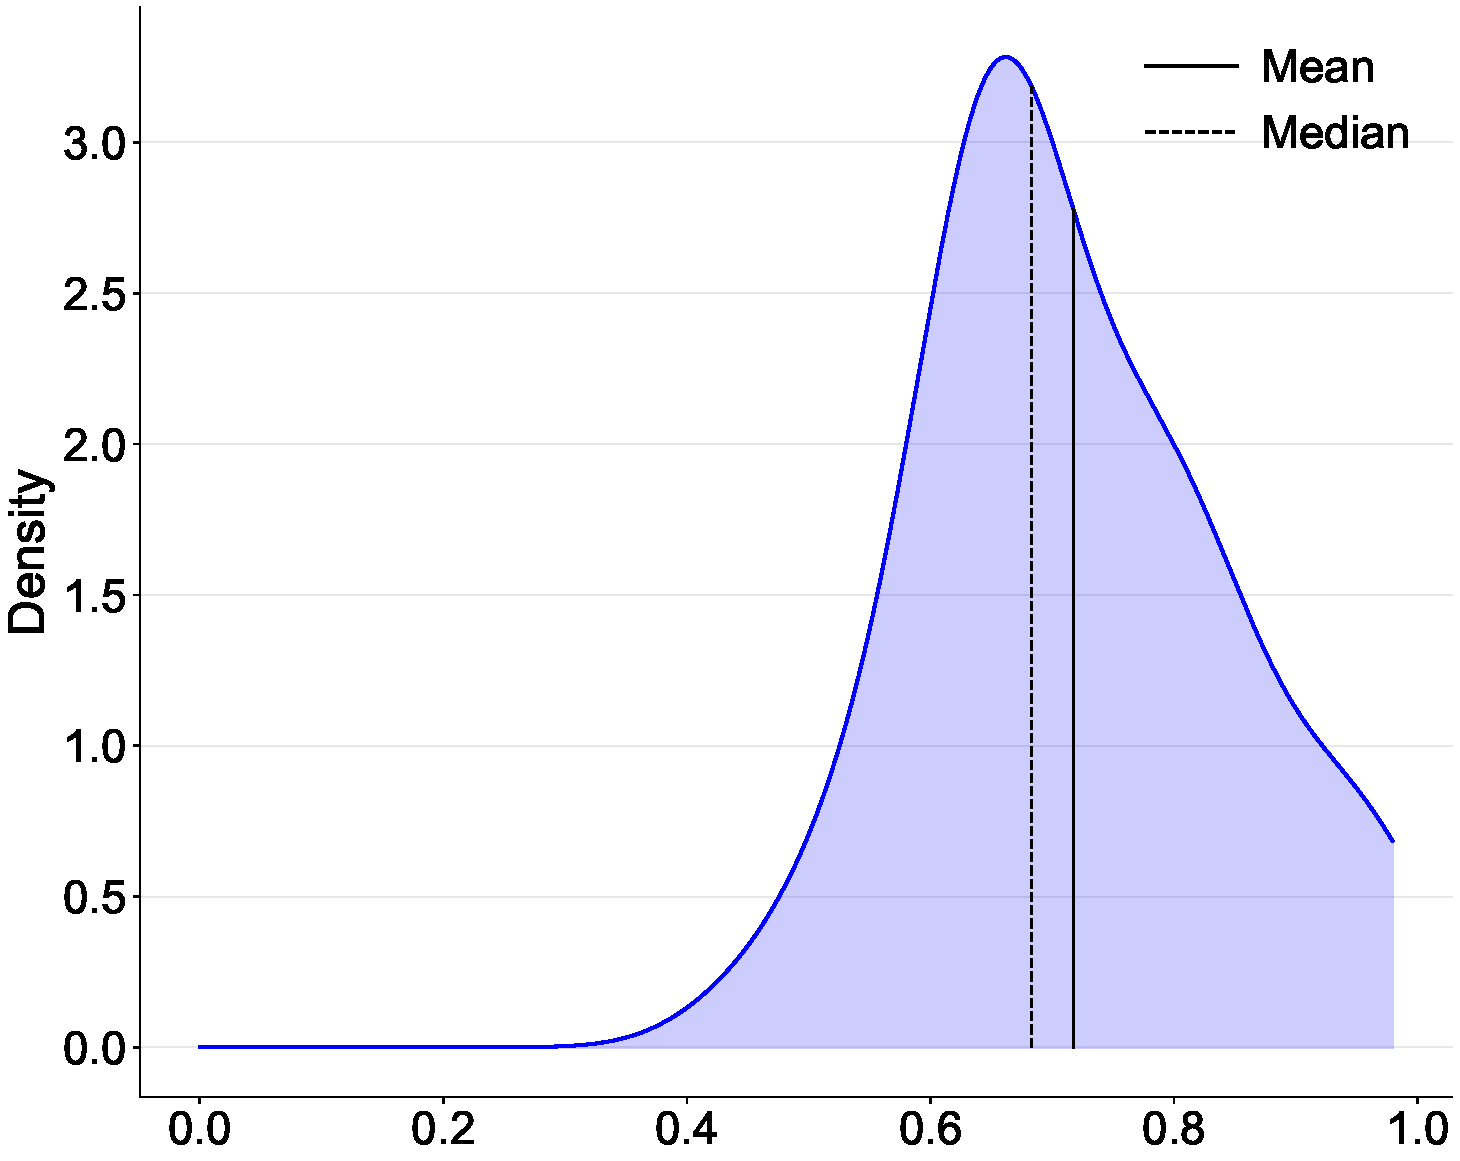
\includegraphics[width=\linewidth]{figures/lime_directionality_1.pdf}
        \caption{{\color{blue}LIME direction alignment}}
    \end{subfigure}
    \hfill
    \begin{subfigure}[t]{0.48\textwidth}
        \centering
        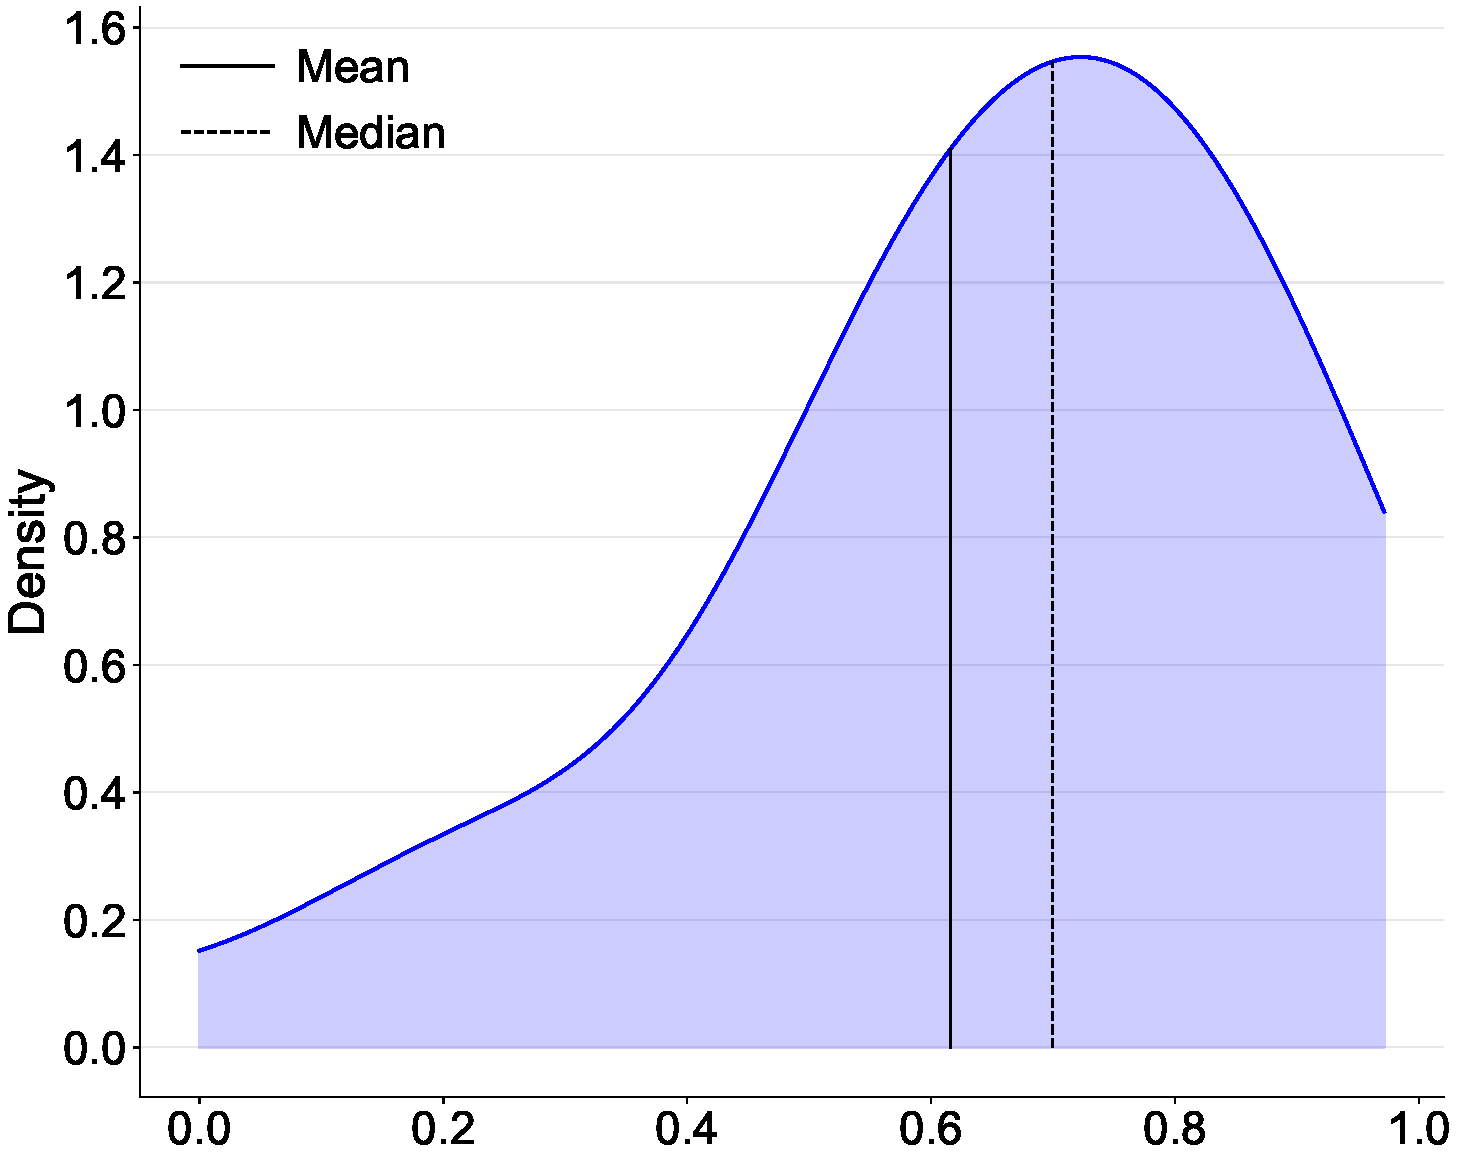
\includegraphics[width=\linewidth]{figures/lime_strength_1.pdf}
        \caption{{\color{blue}LIME strength alignment}}
    \end{subfigure}
    \caption{{\color{blue}\textbf{[Task 1 modification]} Exact Figure~3 distributions under the common ground-truth target.}}
\end{figure}

These baselines give the reader the two comparison points the review team asked for. The naive regression is the floor: on data-generating processes with nonlinearity and interactions, its direction alignment (0.758) falls well below the explanation pipeline's, so the misalignment we document cannot be escaped by simply reverting to a linear model---the difficulty of recovering data-level structure without identifying assumptions is real, and is shared by any such method. FME is the model-side reference: with no explainer in the loop it reaches 0.972 direction alignment, so the fitted models recover direction almost perfectly, and the gap down to {\color{blue}\textbf{[Task 1 modification]} SHAP (mean direction alignment 0.821) and LIME (mean direction alignment 0.717)} is the explainer layer's own contribution to the failure. Partial dependence, which marginalizes over correlated covariates, sits in between (0.810).

To make the size of the failures concrete, we added two interpretable metrics. First, a population-level (aggregate) direction variant: the sign of the average explainer-implied change matches the sign of the average true change in 90.1\% of dataset--feature comparisons for SHAP and 91.4\% for LIME---even under the aggregate notion of directionality that researchers typically invoke, roughly one population-level sign reading in ten is wrong. Second, magnitude accuracy: relative to the mean-absolute attributions the same explainer produces on $\mathcal{G}$, SHAP magnitudes are off by 28\% on average (median 22\%; NRMSE 0.23/0.21) and LIME magnitudes by 34\% (median 29\%; NRMSE 0.28/0.26)---so magnitudes are misestimated by roughly a quarter to a third even when rankings are largely recovered.

\tw{Still to add for this point: the managerial-consequences vignette (retention-budget regret example) and the plain-language translation of alignment scores.}
}
\end{reply}


\begin{aed}
The novelty and the literature claim need to be stated more precisely. The review team has consistently noted that many limitations of SHAP and LIME are already known. The paper will be strongest if it can zero in on where these methods are actually being misused in the business literature and what the present paper adds beyond existing critiques. The distinction between a known limitation of an explainer and an unsupported data-level interpretation needs to be exact. The prevalence claims should also be framed carefully, particularly because the rate is considerably lower in leading journals. Because the paper directly identifies and critiques prior studies, I would also conduct a complete recheck of every paper, quotation, classification, and conclusion. The authors of those papers will scrutinize these claims closely. The analysis needs to be fully accurate, fair, and defensible.
\end{aed}

\begin{reply}

\end{reply}


\begin{aed}
The Rashomon set diagnosis is the most promising part of the paper. It may also provide the clearest basis for a distinctive contribution. At present, however, it remains more of an interesting empirical result than something a practitioner or researcher can readily use. The paper needs to make its practical value much clearer. Can this diagnosis be developed into something that a researcher can apply when evaluating explanations in an actual study? The paper also needs to distinguish this idea carefully from existing work on model multiplicity, explanation instability, and disagreement across near-optimal models.
\end{aed}

\begin{reply}

\end{reply}


\begin{aed}
I agree with the reviewers that there are still important inconsistencies in the paper. Some appear within the main paper. Others appear between the main paper and the appendix. There are also inconsistencies involving the figures, model sets, reported results, terminology, and the ordering of the empirical analyses. These issues make parts of the paper difficult to follow and make some findings difficult to reconcile. Please take the detailed reviewer comments on this point seriously. The authors should conduct a full consistency check of the main paper, the appendix, the analyses, the figures, the captions, and all reported results. The paper would also benefit from further streamlining and another thorough proofreading pass.
\end{aed}

\begin{reply}

\end{reply}


\begin{aed*}
This is shaping up to be an impactful paper. The revision has moved it forward substantially. Still, addressing these points and the review team's concerns would make the contribution much sharper and the final paper much more defensible.
\end{aed*}

\begin{reply}

\end{reply}


\reviewersection{}

\textsf{For ease of reference, we copy your original comments here, in \emph{italics} font.}

\begin{point*}
I enjoyed reading the paper and learned from it. Thank you for a thoughtful and interesting contribution!
\end{point*}

\begin{reply}

\end{reply}

\noindent \textbf{Additional Questions:}

\begin{point*}
Please provide a short summary of what you see as the key argument in the paper.: The paper argues that post hoc explainers such as SHAP and LIME, though intended to explain model predictions, are frequently used for data-level inference---and are not reliable for recovering the direction or strength of relationships between covariates ($\mathbf{X}$) and outcomes ($Y$) in the data-generating process.
\end{point*}

\begin{point}
Research question and contribution: Is the question clear? Is it important (why/why not)? What contribution does answering the question represent? Is it significant or incremental?: The research question is mostly clear: the paper asks whether post hoc explainers can recover data-level relationships ($\mathbf{X}$ and $Y$) rather than just explain model predictions ($\mathbf{X}$ and $\hat{Y}$). However, it is not clear what a positive answer would look like---that is, under what conditions these methods would be considered ``reliable enough,'' and relative to what benchmark. There is no alternative or baseline to interpret the magnitude and practical significance of the reported misalignment.

The question is important because many researchers and practitioners use SHAP and LIME to draw conclusions about the data-generating process, so evaluating the validity of this practice is highly relevant.
\end{point}

\begin{reply}
{\color{red}
The revision supplies the missing comparison points: three baseline estimators---standardized OLS, partial dependence, and forward marginal effects---are now scored under the identical direction and strength metrics on the same 81 data-generating processes. The headline contrast: naive OLS attains mean direction alignment of 0.758, well below {\color{blue}\textbf{[Task 1 modification]} SHAP's exact mean direction alignment of 0.821}, while FME (the fitted model perturbed directly, with no explainer in the loop) attains 0.972; the reported SHAP/LIME alignment levels can now be read against both a floor and a model-side reference. Full results and interpretation appear in our replies to R1.\tw{x-ref R1.3--R1.5} and AE Point 2.
}
\end{reply}


\begin{point}
The contribution is therefore potentially significant, but its impact depends on the ``so what.'' The paper convincingly highlights limitations, but it doesn't clearly articulate what researchers should do instead. Should they rely on simpler models or alternative interpretability tools? Clarifying this would strengthen the practical significance of the contribution. At the same time, the discussion of the Rashomon effect and the use of explanation agreement as a diagnostic are insightful and helpful for thinking about when such explanations can be trusted in practice.
\end{point}

\begin{reply}

\end{reply}


\begin{point}
Method: Is the method used well justified for the question? Is the method applied convincingly (if not, why not)? Does it produce convincing/robust results that answer the question?: The method is well aligned with the research question, and the paper convincingly shows limitations of post hoc explainers. My main concern is with the evaluation---both in how to interpret the significance of the results and in how alignment is measured.

The most important limitation is the absence of a meaningful benchmark. The paper evaluates whether SHAP and LIME recover data-level relationships, but without comparing them to established methods, it is difficult to assess whether the observed misalignment is large or small, and what its practical implications are. This is important because recovering relationships between covariates and outcomes is a long-standing problem in statistics and econometrics, for which many tools already exist. At a minimum, including a simple baseline---such as linear regression with normalized features---would make the results more interpretable. Partial dependence (i.e., marginal effects based on ML models) would also be a useful benchmark.
\end{point}

\begin{reply}
{\color{red}
Both suggested baselines are implemented, plus a third that completes the decomposition. On the same 81 data-generating processes, under the identical metrics:

\begin{itemize}[leftmargin=2em]
\item \textbf{OLS with standardized features:} mean direction alignment 0.758 (median 0.765); mean strength alignment 0.738 (median 0.779). Because most of our DGPs contain nonlinearity and interactions, the misspecified linear model is the floor of the comparison: reverting to a simple regression does not avoid the misalignment problem, it worsens it.
\item \textbf{Partial dependence (Friedman 2001):} mean direction alignment 0.810 (median 0.815); mean strength alignment 0.885 (median 0.927), using the standard deviation of the PD curve as its importance measure (Greenwell et al.\ 2018). PD marginalizes over correlated covariates and evaluates the model off the data manifold, which is visible in its direction score.
\item \textbf{Forward marginal effects (FME; Scholbeck et al.\ 2024):} mean direction alignment 0.972 (median 0.975); mean strength alignment 0.853 (median 0.903). FME perturbs the fitted model directly---no surrogate, no attribution scheme---so it is the reviewer's ``marginal effects based on ML models'' in its purest form, and it doubles as the reference that isolates what the explainer layer adds: the same fitted models whose SHAP/LIME explanations err on direction recover it almost perfectly when interrogated directly.
\end{itemize}

A summary table comparing all five methods appears in our reply to AE Point 2\tw{cross-ref; and add pointer to revised manuscript section once written}.
}
\end{reply}


\begin{point}
For direction, the proposed metric evaluates alignment at the individual level and then averages across instances (Eq.~6). But most of the time researchers care about overall directional relationships, that is, whether a feature is generally increasing or decreasing in its association with the outcome. The current metric instead captures average \emph{local} directional consistency, which is a different object, and may therefore overstate misalignment in terms of how directionality is typically interpreted in practice. A more appropriate measure would assess direction at the aggregate level---for example, by comparing the average direction implied by the explainer (averaging Eq.~2) with the average direction in the DGP (Eq.~3) and evaluating whether their signs agree.
\end{point}

\begin{reply}
{\color{red}
We implemented the aggregate variant exactly as proposed: for each dataset--feature pair, the explainer-implied changes and the true changes are averaged over all evaluation instances and perturbations, and the two signs are compared. Under this population-level criterion the signs agree in 90.1\% of comparisons for SHAP and 91.4\% for LIME. The reviewer's intuition is confirmed---the aggregate scores are higher than the instance-level ones, so the instance-level metric is indeed the stricter notion---but the practical risk does not disappear: roughly one population-level sign reading in ten is still wrong, under precisely the notion of directionality researchers typically report. We present the two metrics together in the revision, the aggregate variant as the one matching common research practice and the instance-level metric as the stricter standard. (Each aggregate comparison is binary, so these results are reported as agreement proportions rather than densities.)
}
\end{reply}


\begin{point}
For strength, I don't think rank correlation alone is enough to capture alignment. A method can recover rankings well while misestimating magnitudes, or vice versa. In many cases, magnitude is what matters: if differences in strength are small, some misranking may not matter much because researchers would still select a reasonable set of features. Conversely, a correct ranking may not be very useful if the underlying magnitudes are poorly estimated or economically negligible. Including another metric that captures magnitude accuracy---such as mean absolute percentage error (MAPE)---would provide a more complete and interpretable assessment.
\end{point}

\begin{reply}
{\color{red}
We adopted the suggestion, reporting MAPE together with normalized RMSE as a bounded companion. Comparing each explainer's mean-absolute attributions under the fitted model against those the same explainer produces on the true data-generating process: SHAP magnitudes deviate by 28\% on average (median 22\%; NRMSE 0.23 mean, 0.21 median), and LIME magnitudes by 34\% (median 29\%; NRMSE 0.28 mean, 0.26 median). The reviewer's conjecture is therefore borne out empirically: rankings can be largely recovered while magnitudes are off by a quarter to a third, so rank correlation alone understates the room for misinterpretation.

One definitional point the revision makes explicit: a Shapley value is a share of a prediction's departure from its baseline, not a rate of change, so a percentage error against average partial effects is well defined for the regression, PD, and FME baselines but not for SHAP; the magnitude comparison above therefore uses each explainer's own magnitude scale (attributions under $\mathcal{M}$ vs.\ under $\mathcal{G}$), and the revised text discusses the estimand distinction directly.\tw{APE-scale MAPE for the baselines + the linear-subset SHAP conversion ($\mathbb{E}|\phi_j| = |\beta_j|\sigma_j\sqrt{2/\pi}$) still to be run; see \S5 of the companion note.}
}
\end{reply}


\begin{point}
Potential impact: Do the results have relevant managerial or policy implications that are potentially important (not necessarily directly, but possibly through a translation), or does the method itself represent a significant innovation? What are the implications? Are they novel and/or significant?: The potential impact depends in part on how SHAP and LIME compare to other alternatives. Without such benchmarks, it is difficult to assess how significant the implications are. That said, the discussion of the Rashomon effect and the idea of using explanation agreement as a diagnostic are quite insightful. These contributions are useful for researchers who rely on post hoc explainers, as they provide practical guidance on when such explanations may be less trustworthy.
\end{point}

\begin{reply}
{\color{red}
The benchmark comparison the reviewer asks for is now in place: SHAP and LIME are evaluated alongside standardized OLS, partial dependence, and forward marginal effects on the same data-generating processes and metrics (see replies to R1.\tw{x-ref R1.3} and AE Point 2). The comparison shows SHAP and LIME are not dominated by the simple alternatives---naive OLS aligns far worse (0.758 direction vs.\ {\color{blue}\textbf{[Task 1 modification]} SHAP's exact mean of 0.821})---while the FME contrast quantifies the alignment the explainer layer itself gives up. \tw{Rashomon-agreement protocol and calibration figure (the ``when to trust'' guidance) to be added under AE Point 4.}
}
\end{reply}


\begin{point}
Writing: Is the paper written at a level of clarity, articulation, logic, and exposition that is appropriate for a major journal?: The paper is clearly written and has improved in terms of focus and articulation compared to the previous version---kudos to the authors for that. That said, there is still a fair amount of repetition, with several (important) ideas restated too many times. There is still room for streamlining to improve readability.
\end{point}

\begin{reply}

\end{reply}


\begin{point}
I would also encourage the authors to be careful with causal language (e.g., ``feature's impact on''). The analysis is about conditional covariation (given other features), which may or may not admit a causal interpretation depending on assumptions about the data-generating process. Being more explicit about this distinction would help avoid potential confusion.
\end{point}

\begin{reply}

\end{reply}


\begin{point}
I also have a couple of additional suggestions (feel free to ignore if not helpful):

(1) Much of the discussion resonates with Shmueli (2010, To Explain or to Predict). Connecting the paper to that literature could strengthen the framing, particularly around the distinction between predictive performance and explanatory validity.
\end{point}

\begin{reply}

\end{reply}


\begin{point}
(2) I recommend removing or moving Sections 5.3 and 6 to an appendix. Section 5.3 feels somewhat redundant given Section 7.3, and Section 6 could be summarized more briefly (e.g., noting that several attempts to address the misalignment of SHAP and LIME do not substantially resolve the issue).
\end{point}

\begin{reply}

\end{reply}


\reviewersection{}

\textsf{For ease of reference, we copy your original comments here, in \emph{italics} font.}

\begin{point*}
The authors have clearly invested substantial effort in this revision, and in my view the manuscript has improved meaningfully. In the first round, while I saw value in the paper's central idea, I was skeptical about several aspects of the framing, evaluation, and overall contribution. The revised manuscript addresses a number of these concerns in a serious and thoughtful manner. In particular, I found the substantially revised literature review and the reconceptualization of the evaluation and experimental framework to be important improvements. At the same time, I still have some concerns regarding how several of my comments were addressed, which I detail below.
\end{point*}

\begin{reply}

\end{reply}


\begin{point}
I believe the related work section has improved, and I appreciate that the authors now articulate more explicitly how the focal paper differs from adjacent work. I still do not fully share the authors' position on this point, as I continue to think that the prior work mentioned already implies more of the present paper's conclusion than the revision currently acknowledges. That said, I recognize that this is at least partly a matter of interpretation, and given the authors' clarifications, as well as the Senior Editor's comment, I am comfortable not pressing this point further.
\end{point}

\begin{reply}

\end{reply}


\begin{point}
The revised literature review on the use of post-hoc explanations to infer relationships in the underlying data is now considerably more convincing. I found it helpful that the authors demonstrate that this practice also appears in top-tier journals, even if at lower rates, and I also appreciated the concrete examples cited on page 15. One way to strengthen this part further, in my view, would be to move beyond documenting prevalence and spell out a bit more explicitly why this practice is problematic in substantive managerial terms. The paper would benefit from a brief illustration of the kinds of flawed managerial or policy conclusions that may follow when researchers treat post-hoc explanations as evidence about the true data-generating process. Making this downstream risk more concrete would further strengthen the paper's motivation.
\end{point}

\begin{reply}

\end{reply}


\begin{point}
While I think Sections 4 and 5 represent an improvement overall, and I agree that the shift toward direction and strength alignment is more sensible than the original framework, I still found parts of the presentation of results somewhat difficult to follow. In Figure 3, SHAP appears clearly superior to LIME with respect to both direction and strength alignment. My understanding is that these results are based on the simulations using the best-performing model for each dataset. However, in the next section, where model accuracy is varied, Figure 4 seems to suggest that in the highest-performance bracket SHAP and LIME perform rather similarly on both dimensions. I found this somewhat confusing.
\end{point}

\begin{reply}

\end{reply}


\begin{point}
Part of this confusion may stem from the presentation itself, which I think could be improved considerably. For example, within Figure 4, the y-axis ranges differ across panels even though the underlying quantities appear comparable. I found this unnecessary and somewhat counterproductive, because it makes visual comparison across panels more difficult. The absence of grid lines further reduces readability. More generally, the figure is not sufficiently self-contained: to understand that the numbers shown in the plots are regression slopes, the reader has to rely on the main text. I would encourage the authors to rework the figure so that it is more interpretable on its own. Similar concerns apply to Figures 5, 6, 7, and 8 (in Figure 6 in particular, the varying y-axis ranges are confusing).
\end{point}

\begin{reply}

\end{reply}


\begin{point}
I also encountered points in the text that were hard to follow. For example, on page 25 the authors mention the ``Feature 0'' yet this feature index does not appear in Figure 5 at all. More broadly, I found the structure somewhat suboptimal. The manuscript first presents results based on the best-performing model, then moves to varying model performance, and then returns to best-performing models in the Rashomon analysis. A more linear structure might make the empirical narrative easier to follow.
\end{point}

\begin{reply}

\end{reply}


\begin{point*}
I would also like to note that I very much appreciated the discussion's emphasis that post-hoc explanations may be ill-suited for validating hypotheses, yet still useful for generating them. In particular, I liked that the authors illustrate this point with examples of studies that use explanations in this more exploratory way, thereby highlighting a productive path forward for researchers.
\end{point*}

\begin{reply}

\end{reply}


\begin{point}
Finally, I believe the paper would still benefit from another careful proofreading pass. There are still a number of typos and minor language issues. For example, on page 3, the sentence ``To assess how prevalent this practice is, we conducted a manual review of 181 papers that made substantive SHAP or LIME.'' appears to be missing a phrase (``use of''). Another example, in the caption or subtext of Figure 3, panel (c) says ``direction alighment''.
\end{point}

\begin{reply}

\end{reply}


\reviewersection{}

\textsf{For ease of reference, we copy your original comments here, in \emph{italics} font.}

\begin{point*}
What I liked: you took the prior round seriously and the paper is markedly better. The direction/strength reframing cleanly resolves the earlier feature-importance/marginal-effect confusion, the literature review is now rigorous and journal-anchored, the simulations are far richer, and the Rashomon-agreement diagnostic is a genuinely useful, practitioner-facing idea. The documented misuse examples are compelling.
\end{point*}

\begin{reply}

\end{reply}

\noindent \textbf{Key issues to address, in priority order:}

\begin{point}
Separate identification from explainer behavior. Your central result like in 5.2 is that predictive accuracy does not identify $\mathcal{G}$. This is a model/data property. Clarify what is failing in SHAP/LIME beyond this, ideally with an example where the model recovers the data's associational structure but the explainer still misleads.
\end{point}

\begin{reply}
{\color{red}
The new forward marginal effects (FME) baseline provides exactly this separation. FME perturbs the fitted model directly---no explainer in the loop---so Oracle$\to$FME measures what the model and data fail to identify, and FME$\to$SHAP/LIME measures what the explanation layer adds on top. The result: across the 81 datasets (best model per dataset), FME attains mean direction alignment of 0.972 (median 0.975), while {\color{blue}\textbf{[Task 1 modification]} SHAP reaches a mean direction alignment of 0.821 (median 0.823) and LIME reaches 0.717 (median 0.683)} for the same models against the same common ground-truth reference. The models recover the data's directional structure almost perfectly; the explainers, applied to those same models, degrade it. This is the requested case in population form: the model recovers the associational structure, and the explainer still misleads. \tw{The cleaner limiting version---applying SHAP/LIME directly to $\mathcal{G}$ (the E1 experiment, where approximation error is zero by construction and any misalignment is explainer-intrinsic) and the correctly specified fitted-model companion---is planned; results to be added here.}
}
\end{reply}


\begin{point}
Define $\mathbf{X} \mapsto Y$ precisely as associational or causal and use it consistently; the contribution reads very differently under each.
\end{point}

\begin{reply}

\end{reply}


\begin{point}
Position the Rashomon-agreement diagnostic against existing model-multiplicity / variable-importance-instability / predictive-multiplicity literature so its novelty is unambiguous.
\end{point}

\begin{reply}

\end{reply}


\begin{point}
Frame the prevalence finding candidly: misuse is far less common in top journals, which bears on how you motivate the paper's urgency for this audience.
\end{point}

\begin{reply}

\end{reply}


\begin{point}
Minor: consider a compact notation table; add a benchmark estimator contrast on the same DGP.
\end{point}

\begin{reply}
{\color{red}
Both are done. A notation table now appears in Section~\tw{ref; add once drafted}. The benchmark contrast is implemented on the same DGPs and metrics---standardized OLS (mean direction alignment 0.758, mean strength alignment 0.738), partial dependence (0.810, 0.885), and forward marginal effects (0.972, 0.853)---with the full comparison and its reading in our replies to R3.\tw{x-ref R3.7} and AE Point 2.
}
\end{reply}

\noindent \textbf{Additional Questions:}

\begin{point*}
Please provide a short summary of what you see as the key argument in the paper.: The paper studies a popular practice in business research and its caveats: interpreting post hoc explainers like SHAP and LIME of a fitted model's behavior as if they revealed the true relationship in the data. The authors did a systematic review of existing studies and show that such ``explanation-as-evidence'' interpretation is common. They introduce two metrics about direction alignment and strength alignment and use simulated data with known ground truth to test whether SHAP/LIME recover the direction and relative importance of features. Their central finding is that explanations look reasonable on average but are highly heterogeneous and can fail even when predictive accuracy is high, with feature correlation and the Rashomon effect (i.e., many equally accurate models that attribute differently) identified as key drivers. They reframe earlier ``mitigation strategies'' as robustness checks and propose Rashomon agreement as a practical reliability measure about the consistency of explanations across equally accurate models. The conclusion is that treat post hoc explanations as hypothesis generators, not as confirmatory evidence about data.
\end{point*}

\begin{point}
Research question and contribution: Is the question clear? Is it important (why/why not)? What contribution does answering the question represent? Is it significant or incremental?: The question is clear and important, and the revision has substantially sharpened it relative to the prior round, especially the original problem of feature importance vs marginal effect conflation. The literature review is now anchored to recognized journal lists and cross-coded with an LLM, which is a real improvement in rigor.

My remaining remark is about the nature of the contribution. As the paper itself now frames it, the gap between model-level explanations and data level truth arises because ``the accuracy of $\mathcal{M}$ does not uniquely identify the underlying structure of $\mathcal{G}$.'' That is fundamentally a statement about model bias and identification, which are fundamental properties of the model class and the data's correlation structure, not about a defect in how SHAP or LIME compute attributions. But the distinctive failure mode here is not ordinary confounding, it is predictive (Rashomon) multiplicity: many equally accurate flexible models yield different explanations, so accuracy fails to select among them. This is exactly what separates the black-box explainability pipeline from direct estimation: a correctly specified regression returns a unique estimate and (for an associational target) recovers the population relationship, whereas the post hoc explanation workflow need not. The paper should make this explicit in its contribution, since otherwise the result reads as a restatement of the well-known prediction vs inference gap. The contribution is significant if the authors can isolate what is genuinely specific to post hoc explainers beyond this generic identification problem; as written, a reader can come away feeling the core result is an XAI-flavored restatement of omitted-variable/identification concerns.

Two concrete asks would resolve this:

State precisely whether ``$\mathbf{X} \mapsto Y$'' denotes the associational DGP or a causal effect. The argument, and its novelty, differ sharply between the two readings.

Show a case where the model faithfully recovers the data's associational structure yet the explainer still misleads. This would demonstrate an explainer-specific failure rather than a model/identification failure.
\end{point}

\begin{reply}
{\color{red}
On the estimand: the revision declares $\mathbf{X}\mapsto Y$ strictly associational---the objects of interest are ceteris paribus properties of the conditional expectation under $\mathcal{G}$---and sweeps the manuscript for causal language accordingly.

On the requested demonstration: the new forward marginal effects baseline supplies its population form. Interrogating the fitted models directly (no explainer in the loop) yields mean direction alignment of 0.972; SHAP and LIME applied to those same models yield {\color{blue}\textbf{[Task 1 modification]} mean direction alignments of 0.821 and 0.717, respectively}. The models recover the data's directional structure nearly perfectly, and the explanation layer demonstrably gives part of it back---an explainer-specific failure, separated from the identification failure the reviewer correctly attributes to the model/data side. \tw{The sharper single-case version (explainers applied directly to $\mathcal{G}$, where $\mathcal{M}=\mathcal{G}$ exactly, plus a correctly specified fitted model that is then misexplained) is planned as experiment E1/3C; add results when available.}
}
\end{reply}


\begin{point}
Method: Is the method used well justified for the question? Is the method applied convincingly (if not, why not)? Does it produce convincing/robust results that answer the question?: The methodology is much stronger than the prior version: richer DGPs (nonlinearity, interactions, correlation, noise), a search across model families rather than a single neural net, and population-level (mean-absolute) strength metrics. The simulation design with known ground truth is appropriate and well executed, and the honesty about long-tailed misalignment even at high accuracy is a genuine strength.

The one methodological point I would press concerns the framing of ``accurate but misaligned''. The result bites only because ``accurate'' means predictive accuracy, which is silent about attribution under correlated features. This is correct and worth making, but the manuscript should state openly that the phenomenon is a consequence of predictive accuracy not constraining attribution, i.e., a model/data identification property surfaced through the explainer. I would also encourage at least one benchmark contrast (e.g., what a correctly specified regression recovers on the same DGP) so readers can see that the failure is shared by any method that does not impose identifying assumptions, which sharpens rather than weakens the paper's message.
\end{point}

\begin{reply}
{\color{red}
The revision states this openly and now demonstrates it: predictive accuracy does not constrain attribution, and the misalignment is shared by any method that does not impose identifying assumptions. The benchmark contrast is implemented on the same DGPs under identical metrics. A naive standardized regression---generically misspecified on our nonlinear, interacting DGPs---attains mean direction alignment of 0.758 and mean strength alignment of 0.738, well below the explanation pipeline, exactly the ``shared failure'' the reviewer predicts. Partial dependence reaches 0.810/0.885, and forward marginal effects (the fitted model perturbed directly) 0.972/0.853; the FME row localizes what the explainer layer alone gives up (see reply to R3.\tw{x-ref R3.1}). \tw{The correctly specified oracle regression per DGP---the unique-estimate upper bound the reviewer describes---is planned; add its numbers here so the floor (naive OLS) and ceiling (oracle) bracket the pipeline.}
}
\end{reply}


\begin{point}
Potential impact: Do the results have relevant managerial or policy implications that are potentially important (not necessarily directly, but possibly through a translation), or does the method itself represent a significant innovation? What are the implications? Are they novel and/or significant?: The managerial relevance is real. SHAP is ubiquitous on ML platforms and is routinely read as substantive evidence, and the four documented examples in Appendix A are quite persuasive. The Rashomon-agreement diagnostic is the most promising and actionable idea in the paper and the clearest candidate for a novel contribution.

However, the novelty of the diagnostic needs positioning against existing work on model multiplicity and importance instability. The related-work treatment of Rashomon cites Breiman, Semenova et al., and Rudin et al., and the robustness section credits Donnelly et al.\ for cross-model averaging, but the paper does not engage the strand that has already proposed using agreement/disagreement across near-optimal models as a reliability signal (e.g., model-class reliance and variable-importance ``clouds,'' predictive multiplicity). Without that positioning, a reader cannot tell how much of section 7 is new versus a re-derivation. I recommend an explicit comparison.
\end{point}

\begin{reply}

\end{reply}


\begin{point*}
Writing: Is the paper written at a level of clarity, articulation, logic, and exposition that is appropriate for a major journal?: The paper is clearer and better organized than the prior submission, and the conceptual progression is easy to follow.
\end{point*}

\begin{reply}

\end{reply}


\end{document}
